\documentclass[12pt,a4paper]{article}

\usepackage[brazil]{babel}
\usepackage[utf8]{inputenc}
\usepackage[T1]{fontenc}
\usepackage{graphicx}
\usepackage{epsfig}
\usepackage{cite}
\usepackage{verbatim}
\usepackage{concrete}
\usepackage{amsfonts}
\usepackage{amsmath}
\usepackage{amssymb}
\usepackage{setspace}
\usepackage{url}
\usepackage{subfigure}
\usepackage{array}
\usepackage{multirow}
\usepackage{colortbl}
\usepackage{tabularx}
\usepackage{geometry}
\usepackage{cite}
\usepackage{xcolor}
\usepackage{color}
\usepackage{url}
\usepackage{lmodern}
\usepackage{pict2e}
\usepackage{siunitx}

\geometry{top=2.3cm,bottom=2.2cm,left=2.5cm,right=2.5cm}

\newcommand{\V}[1]{\boldsymbol{#1}}

\providecommand{\todo}[1]{{\textbf{\protect\color{red} {TODO: #1}}}}

\newenvironment{myitemize}{
\begin{itemize}
 \setlength{\itemsep}{1pt}
 \setlength{\parskip}{0pt}
 \setlength{\parsep}{0pt}
}{\end{itemize}}

\newenvironment{myenumerate}{
\begin{enumerate}
 \setlength{\itemsep}{1pt}
 \setlength{\parskip}{0pt}
 \setlength{\parsep}{0pt}
}{\end{enumerate}}

%  ABACO -- Conjunto de macros para desenhar o 'abaco

%  Desenho original de Hans Liesenberg

%  Macros de Tomasz Kowaltowski

%  DCC -- IMECC -- UNICAMP

%  Mar,co de 1988  --  Vers~ao 1.0

% Ajustado para LaTeX da SUN -- Mar,co de 1991

% ---------------------------------------------------------

%  Chamada:   \ABACO{d1}{d2}{d3}{d4}{esc}
%             com:  di's -- os quatro d'igitos;
%	           esc  -- fator de escala

% ---------------------------------------------------------

%  DEFINI,C~OES AUXILIARES

% ---------------------------------------------------------


%  Forma o d'igito pequeno (0 ou 1)

\newcommand{\ABACODP}[1]{%
%
\thicklines
%    
\begin{picture}(8,0)
    \ifcase#1{   %  caso 0
       \put(0,0)    {\line(1,0){4}}
       \multiput(5,0)(2,0){2}{\oval(2,4)}}
    \or{         %  caso 1
       \put(2,0)    {\line(1,0){4}}
       \multiput(1,0)(6,0){2}{\oval(2,4)}}
    \fi
\end{picture}
    } % \ABACODP

% Forma o d'igito grande (0 a 4)

\newcommand{\ABACODG}[1]{%
%
\thicklines
%    
\begin{picture}(14,0)
    \ifcase#1{   % caso 0
       \multiput(1,0)(2,0){5}{\oval(2,4)}}
       \put(10,0)   {\line(1,0){4}}
    \or{         % caso 1
       \multiput(1,0)(2,0){4}{\oval(2,4)}}
       \put(8,0)   {\line(1,0){4}}
       \put(13,0)   {\oval(2,4)}
    \or{         % caso 2
       \multiput(1,0)(2,0){3}{\oval(2,4)}
       \put(6,0)   {\line(1,0){4}}
       \multiput(11,0)(2,0){2}{\oval(2,4)}}
    \or{         % caso 3
       \multiput(1,0)(2,0){2}{\oval(2,4)}
       \put(4,0)   {\line(1,0){4}}
       \multiput(9,0)(2,0){3}{\oval(2,4)}}
    \or{         % caso 4
       \put(1,0)  {\oval(2,4)}}
       \put(2,0)   {\line(1,0){4}}
       \multiput(7,0)(2,0){4}{\oval(2,4)}
    \fi
\end{picture}
    } % \ABACODG
       
% Forma um d'igito (0 a 9)

\newcommand{\ABACOD}[1]{%
%
    \ifnum#1>9
       \errmessage{#1: Argumento invalido para ABACO}
    \fi
    \ifnum#1<0
       \errmessage{#1: Argumento invalido para ABACO}
    \fi
%
\begin{picture}(24,0)
%    
    \ifnum#1<5
       \put(16,0) {\ABACODP{0}}
    \else   
       \put(16,0) {\ABACODP{1}}
    \fi
%    
    \ifnum#1<5
       \put(0,0)  {\ABACODG{#1}}
    \else
       \ifcase#1\or \or \or \or
          \or  \put(0,0)  {\ABACODG{0}}
          \or  \put(0,0)  {\ABACODG{1}}
          \or  \put(0,0)  {\ABACODG{2}}
          \or  \put(0,0)  {\ABACODG{3}}
          \or  \put(0,0)  {\ABACODG{4}}
       \fi
    \fi   
\end{picture}
    } % \ABACOD
    
% -------------------------------------------------

%  DEFINI,C~AO PRINCIPAL
    
\newcommand{\ABACO}[5]{%
    \setlength{\unitlength}{#5mm}
%
    \thinlines
%   
\begin{picture}(28,25)
%   
% moldura
%
% externa
%
        \put(0,0)            {\line(0,1){25}}
        \put(0,0)            {\line(1,0){28}}
        \put(28,0)           {\line(0,1){25}}
        \put(0,25)           {\line(1,0){28}}
% interna
        \put(2,2)            {\line(0,1){21}}
	\put(26,2)           {\line(0,1){21}}
	\put(16,2)           {\line(0,1){21}}
	\put(18,2)           {\line(0,1){21}}
	\put(2,2)            {\line(1,0){14}}
	\put(16,2)           {\line(1,-1){1}}
	\put(17,1)           {\line(1,1){1}}
	\put(18,2)           {\line(1,0){8}}
	\put(2,23)           {\line(1,0){14}}
	\put(16,23)          {\line(1,1){1}}
	\put(17,24)          {\line(1,-1){1}}
	\put(18,23)          {\line(1,0){8}}
	\put(0,0)            {\line(1,1){2}}
	\put(0,25)           {\line(1,-1){2}}
	\put(28,0)           {\line(-1,1){2}}
	\put(28,25)          {\line(-1,-1){2}}
%
%   
% d'igitos
%
%   
       \put(2,20)  {\ABACOD{#1}}
       \put(2,15)  {\ABACOD{#2}}
       \put(2,10)  {\ABACOD{#3}}
       \put(2,5)   {\ABACOD{#4}}
%      
\end{picture}
    } % \ABACO
    


\begin{document}

\tolerance = 999
\sloppy

\hyphenation{re-co-nhe-ci-men-to}
\hyphenation{ca-rac-te-rís-ti-cas}
\hyphenation{a-pre-sen-ta-ção}
\hyphenation{pos-si-bi-li-ta-rá}

\thispagestyle{empty}

\begin{center}{\large \bf UNIVERSIDADE ESTADUAL DE CAMPINAS} \end{center}
\begin{center}{\large INSTITUTO DE COMPUTAÇÃO} \end{center}

\begin{center}
\begin{minipage}[tl]{31mm}
  \ABACO{1}{9}{6}{9}{1}
\end{minipage}
\end{center}

\vspace*{3.5cm}

\begin{center}
{\Large \bf MC833 - Relatório Científico 1}

\vspace*{2.0cm}

\textsc{\Large Comunicação Cliente-Servidor} \\ [0.1cm]
\textsc{\Large Usando Protocolo TCP}

\vspace{2.5cm}

\textbf{135368:} Cristina Freitas Bazzano \\
\textbf{135749:} Flávio Altinier Maximiano da Silva

\vspace{7.5cm}

{\large Campinas - SP}
\vspace*{0.2cm}

{\large Abril de 2015}
\end{center}

\clearpage

\pagenumbering{arabic}
\onehalfspacing
\tableofcontents 
\clearpage
\onehalfspacing

\begin{abstract}
Este trabalho focou-se no estudo temporal de redes cliente-servidor baseadas em comunicação TCP. Foi implementado um serviço de locadora de filmes baseado em {\it MySQL} no servidor, e ao cliente foram adicionadas diversas operações de acesso ao banco, baseando-se em operações de consultas pequenas, grandes e de escrita. Observou-se que a escrita no banco é o processo mais lento, enquanto operações de consultas extensas são apenas brevemente mais lentas que buscas mais curtas. Outro ponto interessante medido foi a confiabilidade das transmissões e, conforme prometido pelo protocolo TCP, todas as mensagens foram recebidas corretamente. Além disso, uma breve análise de tamanho de código mostrou que operações de redes não são as mais presentes em uma implementação desse tipo.
\end{abstract}

\section{Introdução}
Na Internet, a grande maioria das montagens de comunicação baseia-se em um sistema cliente-servidor. Nesse contexto, o servidor guarda alguma informação que é relevante ao cliente, que pede essa informação através de uma mensagem na rede; o servidor, por sua vez, responde esse pedido com outra(s) mensagem(ns) contendo a informação requisitada.

O protocolo da camada de transporte escolhido para este projeto é o {\it Transmission Control Protocol} (TCP)~\cite{postel1981transmission}. Tal protocolo garante que as mensagens enviadas por um host cheguem sem alterações (se o conteúdo da mensagem não corresponder ao {\it checksum}, ela é re-enviada), além de garantir que as mensagens chegam em ordem. Num trabalho futuro, faremos as análises usando também o {\it User Datagram Protocol} (UDP)~\cite{postel1980user} e compararemos os resultados.

Neste trabalho, num primeiro momento, o foco principal de nossa análise será a medida de tempo total de comunicação entre cliente e servidor, além de uma aproximação do tempo de transmissão das mensagens entre os dois (tempo de as mensagens saírem de um host e chegarem ao outro). Analisaremos também brevemente a confiabilidade das mensagens enviadas, mas, conforme já especificado, a confiabilidade das mensagens é garantida pelo protocolo. O tamanho de código será também analisado, além de um breve parecer sobre o nível de abstração do sistema desenvolvido.

\section{Descrição Geral do Sistema}

O sistema construído consiste em uma simples montagem de cliente-servidor, com comunicação TCP. Como discutido, tal protocolo garante que as mensagens enviadas entre cliente e servidor cheguem em ordem e exatamente iguais ao conteúdo enviado.

    O sistema montado é uma emulação de um serviço de locadora online, onde o servidor contém diversas informação sobre os filmes que possui em seu estoque, os quais podem ser acessadas por clientes ou pelo cliente administrador da locadora. 
    
    Para sintetizar o problema da melhor forma possível, criamos no nosso banco de dados uma tabela “Locadora” que armazena os seguintes atributos sobre os filmes que possui: título, ano de lançamento, gênero, duração, sinopse, diretor, ator principal, ator coadjuvante principal, exemplares e um id único para cada filme. 
    
Os acessos do cliente ou do administrador da locadora ao servidor são com pedidos de informação ou escrita de dados de cada filme, sendo eles da seguinte forma:

\begin {myenumerate}
\item Listar todos os títulos dos filmes e o ano de lançamento;
\item Listar todos os títulos dos filmes e o ano de lançamento de um gênero determinado;
\item Dado o identificador de um filme, retornar a sinopse do filme;
\item Dado o identificador de um filme, retornar todas as informações deste filme;
\item Listar todas as informações de todos os filmes;
\item Alterar o número de exemplares em estoque;
\item Dado o identificador de um filme, retornar o número de exemplares
em estoque.
\end{myenumerate}

    Todos esses acessos podem ser feitos em dois modos de consulta: um que realiza a consulta apenas uma vez, para testar sua corretude, e outro que realiza a consulta sequencialmente, cada acesso é repetido 30 vezes e todos os tempos são armazenados em um arquivo {\it log}, para possibilitar uma futura análise dos mesmos.
    
    Classificamos esses acessos em 3 categorias: as consultas pequenas, consultas grandes e operações de escrita. De acordo com a consulta que cada operação realiza podemos dividí-las da seguinte forma: no primeiro grupo se encontram as operações de 1 a 4 e a operação 7, no segundo grupo temos apenas a operação 5 e no terceiro grupo temos a operação 6. 
    
O primeiro grupo é caracterizado por uma consulta rápida de até 1500 bytes, que é o tamanho máximo MTU (Maximum Transmission Unit) que um pacote pode ter para ser transmitido pela camada Ethernet. O segundo grupo realiza consultas longas, com mais de 1500 bytes, que devem ser quebradas em mais de um pacote para serem enviadas. E o terceiro grupo é caracterizado por uma consulta que carrega um maior atraso do bando de dados, uma vez que no tempo medido está embutido o tempo de escrita no banco.


\section{Armazenamento e Estruturas de Dados}

Em um sistema real de cliente-servidor os dados são em sua maioria armazenados em Banco de Dados para garantir a persistência e a consistência dos mesmos. Com o objetivo de nos aproximar o máximo possível de um problema real, adotamos o MySQL~\cite{mysql1995mysql} como o Banco de Dados para armazenar os dados da locadora de filmes no servidor.

    Populamos o banco do servidor com dados de 10 filmes retirados do site IMDb~\cite{IMDbsite}, os quais estão classificados com as 10 melhores notas no mesmo. Optamos por uma quantia pequena de exemplares para que os tempos medidos nas operações não fossem totalmente influenciados pelo tempo de acesso ao servidor, visto que os tempos de comunicação são o foco da análise do projeto.
    
    No acesso ao banco de dados, os clientes podem apenas acessar a informação, enquanto o cliente administrador da locadora pode, além do acesso, alterar a quantidade de exemplares em estoque. Para garantir esse privilégio de acesso, é necessário uma senha para entrar no modo administrador, a qual é processada pelo programa e só após confirmada o acesso diferenciado ao banco pode ocorrer.
    
Com o objetivo de fazer um sistema robusto, que garante a confiabilidade do mesmo, optamos por utilizar uma cópia do banco de dados do servidor no lado do Cliente, possibilitando assim uma conferência dos dados retornados pelas consultas. Apesar de ser uma manobra simulada, nos permite confirmar a confiabilidade do protocolo TCP, que para todos os nossos exemplos retornou as consultas em ordem, da forma que foram enviadas pelo servidor. E portanto, essa manobra também nos permitirá dizer se o mesmo ocorre quando utilizamos um protocolo sem confiabilidade, que é o caso do UDP.

\section{Detalhes de Implementação}

Tanto o cliente quanto a servidor foram implementados baseando-se nas descrições encontradas em~\cite{hall19beej}. A porta do servidor escolhida para comunicação foi a porta “35368”.

Para o servidor, o socket de “escuta” é iniciado com o auxílio da operação {\it getaddrinfo()}; o tipo de socket é o SOCK\_STREAM, que caracteriza uma comunicação TCP. Além disso, por ser TCP, após fazer o {\it bind} do socket à porta supracitada, o servidor fica “escutando”, esperando por conexões.

O servidor então entra em um loop infinito, no qual fica “aceitando” novas conexões. Quando recebe um pedido de conexão, faz um {\it fork} e a comunicação com esse cliente é tratada por um processo filho. Dessa forma, garantimos que o servidor aceita outras conexões mesmo quando já está conectado a algum cliente.

No cliente, seguimos a comunicação também como descrito~\cite{hall19beej}: o socket de comunicação também é criado com o auxílio de {\it getaddrinfo()}. Em ambos os casos, como a comunicação é feita em LAN, a função retorna apenas as informações de cliente e servidor diretamente, então não é necessário o loop como feito na literatura~\cite{hall19beej}.

O cliente, a cada vez que é iniciado, joga na tela um {\it prompt} com as opções de requisição ao servidor. Em seguida, após escolhida a opção, o cliente dá a opção de fazer o acesso apenas uma vez (para verificar a corretude da aplicação) ou trinta vezes. Se o usuário escolher por fazer o acesso apenas uma vez, o resultado da consulta é exibido na tela do cliente. Se escolher por fazer a consulta trinta vezes, um arquivo de {\it log} de respostas é criado na mesma pasta do cliente, com o nome {\it testX.txt}, onde {\it X} é o número do teste escolhido pelo usuário no {\it prompt}.

A consulta é feita ao servidor pelo meio de envio de consultas {\it MySQL}, que são montadas no próprio programa do cliente. Essas consultas são enviadas como mensagens ao servidor que simplesmente as aplica ao seu banco de dados e retorna o resultado das consultas de leitura ou escrita, também em forma de mensagens. Essa mesma consulta é aplicada a um banco de dados local no cliente, que é exatamente igual ao do servidor; o resultado local dessa consulta é usado para verificar a confiabilidade do resultado enviado pelo servidor.

Esse arquivo de {\it log} gerado tem o seguinte formato: são trinta linhas e três colunas, onde cada linha representa um dos testes. A primeira coluna representa o tempo total de comunicação entre cliente e servidor (desde o {\it connect()} até o {\it close()}); a segunda dá o intervalo de tempo contado desde imediatamente antes do {\it send()} da consulta até imediatamente após o {\it recv()} do resultado. A terceira coluna traz um valor numérico da seguinte forma: se a mensagem recebida for igual à gerada no banco de dados local, ou seja, se a transmissão foi confiável e as mensagens chegaram corretamente, esse valor é zero. Qualquer outro valor diferente de zero significa que houve corrupção de mensagens.  Como o protocolo de transporte utilizado é o TCP, espera-se que esse valor seja zero para todos os testes. Num próximo experimento, quando utilizaremos UDP como protocolo de transporte, esse valor poderá variar.

O servidor também concatena a um arquivo de {\it log} dados sobre cada conexão que coordena. Como o servidor concatena informações num mesmo arquivo, quando o cliente fizer, por exemplo, trinta consultas de títulos de filmes, as últimas trinta entradas desse {\it log} do servidor guardarão os dados sobre essas consultas. Cada entrada nesse {\it log} é um {\it float} que guarda o tempo de acesso do servidor ao banco de dados; esse tempo é o intervalo desde imediatamente após o {\it recv()} da consulta até imediatamente antes do {\it send()} do resultado. Dessa forma, podemos calcular o tempo de transmissão das mensagens: usando o tempo $ tServer $ desse {\it log} do servidor e a segunda coluna do {\it log} do cliente ($ tClient $), o tempo de transmissão de uma mensagem ao outro será dado por:
\begin{equation}
{\text {Tempo de Transmissão}} = \frac{tClient - tServer}{2}
\label{eqn:time}
\end{equation}
Um outro pequeno detalhe de implementação é que apenas o cliente administrador da locadora deve ter autorização para alterar o número de exemplares em estoque de cada filme. Portanto, quando um cliente decide fazer essa alteração, é perguntado por uma senha. Essa senha é verificada no próprio programa do cliente (é hard-coded como “1234”) e, apenas se estiver correta, o programa continua. Essa escrita no banco de dados também é hard-coded para garantir a consistência entre o banco de dados local e o remoto (do servidor), para que posteriormente possa ser verificada a confiabilidade das mensagens. Numa situação de mundo real, onde não há banco de dados local, essa opção não pode ser hard-coded.

O tamanho máximo de buffer adotado é de um milhão de caracteres; o tamanho máximo das consultas são 150 caracteres. O backlog suportado pelo servidor é de cinco pedidos de conexão.


\section{Análise dos Resultados}

\subsection{Tempo total de Comunicação}

Em todos os resultados dos tempos médios utilizamos um intervalo de confiança com nível de confiança de 95\%, obtido a partir da soma ou subtração de dois desvios padrão.
    
Primeiramente geramos um gráfico com o tempo total de conexão com o servidor para cada uma das operações. O resultado segue demonstrado na Tabela~\ref{table:total} e na Figura~\ref{fig:total}.

\begin{table}[h]
\centering
\caption{Tabela mostrando o tempo médio e intervalo de confiança para cada uma das sete operações, na ordem em que foram descritas. Tempo calculado no cliente, desde a abertura até o fechamento da conexão.}
\label{table:total}
\begin{tabular}{lll}
Operação & Tempo Médio Total (\SI{}{\milli\second}) & Intervalo de Confiança (\SI{}{\milli\second})\\ \hline
1        & 38.42           & 5.59   \\
2        & 37.38           & 9.14   \\
3        & 37.47           & 7.59   \\
4        & 37.10           & 10.37  \\
5        & 40.41           & 9.15   \\
6        & 114.10          & 95.27  \\
7        & 36.49           & 7.88  
\end{tabular}
\end{table}

\begin{figure}[h]
\centering
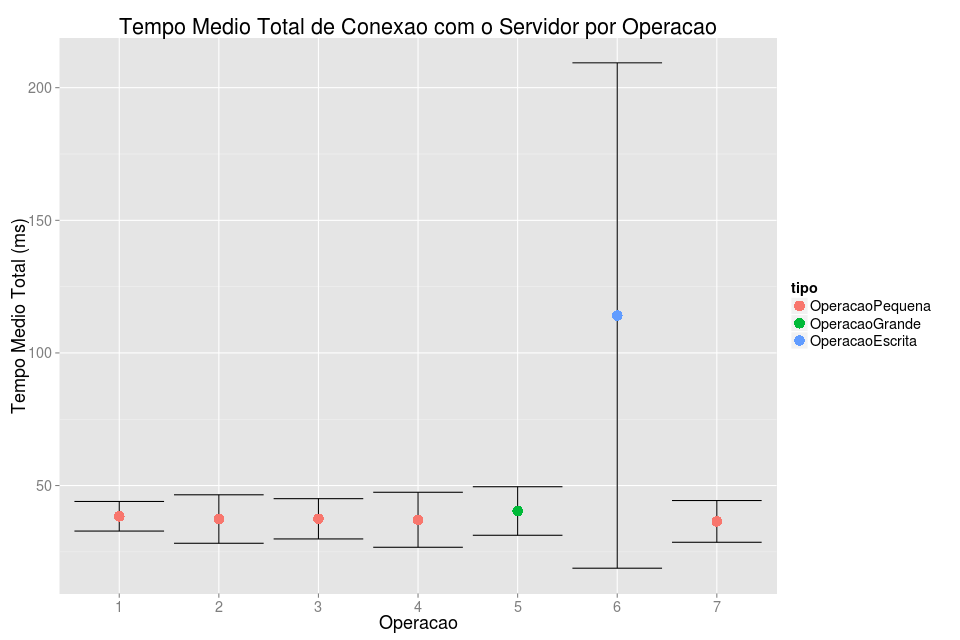
\includegraphics[width=\textwidth]{diagrama/resultadosTempoTotal.png}
\caption{Mostra o tempo médio e o intervalo de confiança de 95\% para as sete operações, na mesma ordem em que foram descritas. Tempo calculado no cliente, desde a abertura até o fechamento da conexão.}
\label{fig:total}
\end{figure}

Os resultados que obtivemos para o tempo total de conexão dependem bastante das consultas ao banco de dados e do tamanho das mensagens. Esses mensagens nas operações pequenas, como já especificado, podem ser totalmente enviadas em apenas um pacote, enquanto nas operações grandes, vários pacotes são necessários para o envio completo das mensagens. Nas operações de escrita, apesar de só um pacote ser necessário para o envio da mensagem, a consulta ao banco de dados para alteração requer um tempo de conexão bem maior do que as consultas de informação. É interessante notar que o desvio da operação de escrita também é consideravelmente maior do que o das outras operações; acreditamos porém que essa variação é causada pelo atraso do banco de dados, e não apenas da rede.

Com isso em mente, os resultados foram como esperado. As operações pequenas estão todas na mesma faixa e a operação grande está apenas um pouco acima destas, visto que a única diferença entre essas duas categorias é a quantidade de pacotes recebidos, que causou um pequeno aumento no tempo medido. Já a operação de escrita apresenta uma grande diferença em relação as demais; o acesso ao banco para alteração de valores gera um {\it overhead} muito grande nesse medida, que acaba representando bem mais o tempo de alteração do banco de dados do que o tempo de conexão com o servidor.

\subsection{Tempo de Transmissão}

Em seguida geramos um gráfico com o tempo total de transmissão das mensagens para cada uma das operações, como explicitado pela equação~\ref{eqn:time}. O resultado segue na Tabela~\ref{table:transmissao} e Figura~\ref{fig:transmissao}.

Os tempos de transmissão medem o tempo de comunicação entre o cliente e o servidor. Esse tempo deve depender apenas do tamanho das mensagens, que como já especificado, corresponde apenas a um pacote nas operações pequenas e de escrita e de vários pacotes nas operações grandes. 

Os tempo obtidos para as operações pequenas e grandes condizem com essa expectativa; o tempo de transmissão da operação grande é levemente maior que o das pequenas. O tempo de transmissão da operação de escrita, porém, fica muito acima do esperado. Assumimos este ser um erro de medida: dado que isto é uma aproximação, o tempo total pode ter influenciado um atraso maior no tempo de transmissão.

\begin{table}[h]
\centering
\caption{Mostra o tempo médio e intervalo de confiança de 95\% para transmissão de mensagens segundo a equação~\ref{eqn:time} para cada uma das operações, na ordem em que foram descritas.}
\label{table:transmissao}
\begin{tabular}{lll}
Operação & Tempo Médio de Transmissão (\SI{}{\milli\second}) & Intervalo de Confiança (\SI{}{\milli\second}) \\ \hline
1        & 11.02                & 2.86   \\
2        & 10.35                & 4.09   \\
3        & 10.79                & 3.30   \\
4        & 10.43                & 4.61   \\
5        & 11.99                & 4.45   \\
6        & 24.19                & 48.88  \\
7        & 10.37                & 3.66  
\end{tabular}
\end{table}

\begin{figure}[h]
\centering
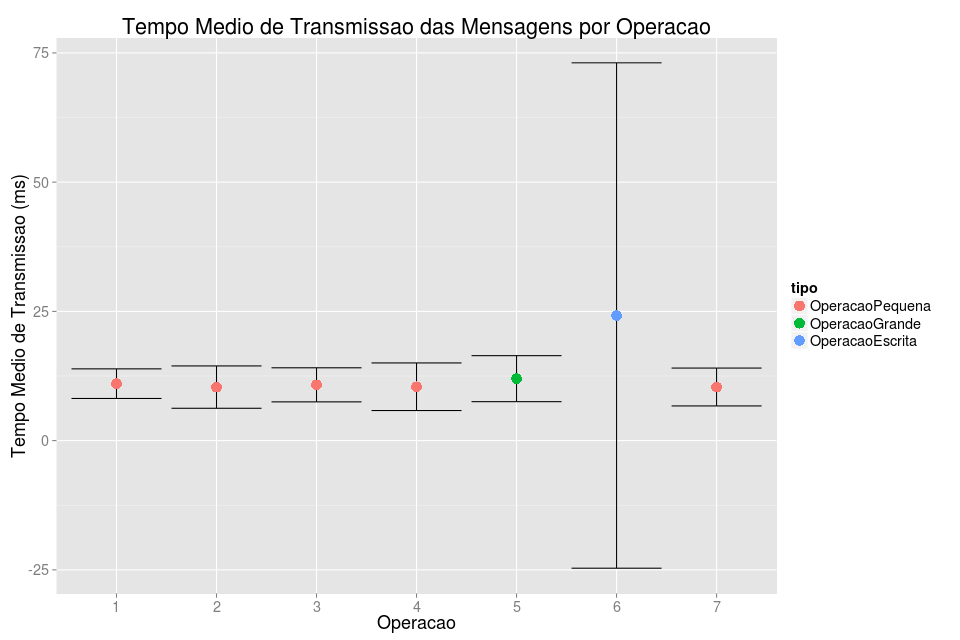
\includegraphics[width=\textwidth]{diagrama/resultadosTempoTransmissao.png}
\caption{Tempo médio, com intervalo de confiança de 95\%, calculado conforme a equação~\ref{eqn:time}, para as sete operações na mesma ordem em que foram descritas.}
\label{fig:transmissao}
\end{figure}

\subsection{Tamanho de Código}
As operações de redes são, na verdade, parte pequena do código total da aplicação. No servidor, a parte mais extensa do código são claramente as operações de consulta {\it MySQL}. No cliente, além das operações de banco de dados, há dezenas de linhas voltadas apenas para a saída na tela dos {\it prompts} ou a escrita em arquivo.

As operações de redes, mesmo no servidor que faz algumas operações a mais que o cliente, representam muito pouco do código. Considerando-se o servidor, as operações de redes mais os seus testes de erros somam 51 linhas, enquanto o arquivo todo tem 191 (correspondem a cerca de 26\%). Para o cliente, as operações de redes representam 31 de um total de 342 linhas (cerca de 9\%). 

\subsection{Confiabilidade}

Como o protocolo escolhido foi o TCP, que garante confiabilidade na transmissão de mensagens, a confiabilidade esperada era de 100\%. De fato, todas as consultas feitas foram exatamente iguais às geradas localmente para contra-prova, comprovando experimentalmente a confiabilidade do protocolo.

\subsection{Nível de Abstração}

As operações de redes fornecidas pelo sistema são bastante abstratas, apesar de algumas exigirem o entendimento de ponteiros e espaços de memória, meros detalhes da linguagem C. O "diálogo" entre cliente e servidor é resolvido com mensagens, e as operações são tão abstratas quanto imaginamos: baseiam-se em processos de envio ({\it send()} e {\it recv()}). Mesmo operações exclusivas a servidores, como {\it bind()} e {\it listen()}, embora não sejam tão instintivas, uma vez entendido o protocolo, fazem sentido e tem boa abstração. 

Em suma, é possível perceber que toda a complexidade do protocolo está escondida atrás de operações simples.

\section{Conclusões}

No sistema cliente-servidor implementado neste projeto a informação que o servidor retém é a do seu banco de dados e todas as mensagens se baseiam em consultas {\it MySQL}. O tempo total está totalmente influenciado pelo tempo de acesso ao banco, como fica visível na operação de escrita.

Devido a característica desta aplicação apenas uma pequena parte do código do sistema realiza as operações de redes. Apesar disso, essas operações são carregadas pela sua abstração, onde toda a complexidade esta embutida apenas em um comando básico. A abstração condiz com o tempo de execução dessas operações, medidos no tempo de transmissão, que equivale a menos de um quarto do tempo total na maioria das operações.

A confiabilidade garantida pelo protocolo TCP utilizado na comunicação do sistema foi comprovada em todas as consultas. Um futuro trabalho será comparar esses resultados com um sistema que utiliza o protocolo UDP, onde a confiabilidade pode não ser tão perfeita.

\addcontentsline{toc}{section}{\protect\numberline{}Referências}

\singlespace
\bibliographystyle{unsrt}
\bibliography{relatorioTCP}

\end{document}
